\section{Φασματική Κατανομή της Ισχύος}

Ο δίσκος θερμοκρασίας $Τ_{dust}$ βρίσκεται σε Θερμοδυναμική Ισορροπία και ακτινοβολεί. Θέλουμε να βρούμε την φασματική κατανομή της ενέργειας του δίσκου, ({\en SED}),  που λαμβάνει παρατηρητής σε απόσταση $D=100 \; pc$ απο τον δίσκο βλέποντας τον {\en ``face on``}, δηλαδή στην \eqref{eq:SpecificIntensity} $\theta=0\deg$. H {\en SED} είναι ένα διάγραμμα $\lambda F_{\lambda}$ {\en vs} $\lambda$, το οποίο χρησιμοποιείται ευρέως για τον χαρακτηρισμό αστρονομικών πηγών.\\
Προκειμένου να υπολογίσουμε την {\en SED} συντάχθηκε ένα {\en script} με την ονομασία {\en {\it System'sSED.py}}, όπου θεωρήσαμε ότι κάθε δακτύλιος του δίσκου αντιπροσωπέυει ένα {\en ``pixel``} πάχους $Dr=0.17AU$. Έτσι το σύνολο των σωματιδίων κάθε δακτυλίου $i=1,2,...,120$, πάχους $Dr_i$, επιφανειακής πυκνότητας $\Sigma_{ri}$ και θερμοκρασίας $Τ_{ri}$ αντιπροσωπεύουν ένα <<μεγάλο σωματίδιο>>.  Ο παρατηρητής σε απόσταση $D$ απο τον δίσκο λαμβάνει, απο κάθε δακτύλιο $i$, μονοχρωματική ροή ακτινοβολίας $F_{\lambda}^i$ (ή $F_{\nu}^i$ αντίστοιχα). Θεωρούμε την ακτινοβολία πίσω απο τον δίσκο αμελητέα$\cdot$ έτσι απο τις σχέσεις \eqref{eq:RadiationTransferEquation4}, \eqref{eq:RadiationTransferEquationBlackBody}, \eqref{eq:SpecInteBlackBody} και \eqref{eq:SpecInteBlackBody2} προκύπτει:

\begin{align}
 F_{\lambda}^i = (\frac{2\pi rDr}{D^2})(1-e^{-\tau_{\lambda}^i})B_{\lambda}(Τ_{dust}^i)\label{eq:MonochromaticFlux}\\
 F_{\nu}^i = (\frac{2\pi rDr}{D^2})(1-e^{-\tau_{\nu}^i})B_{\nu}(Τ_{dust}^i)\nonumber
\end{align}

Η εκπομπή στα μεγάλα μήκη κύματος απο τα σωματίδια της σκόνης έχει μικρό οπτικό βάθος, άρα τα σωματίδια που βρίσκονται μπροστά δεν αποκόπτουν μέρος της ακτινοβολίας αυτών που βρίσκονται πιο πίσω. Ουσιαστικά όπως για την απορρόφηση έτσι και για την εκπομπή θεωρούμε ότι ο δίσκος έχει μικρό οπτικό βάθος ({\en optically thin Disc}). Το οπτικό βάθος,\eqref{eq:OpticalDepth}, δίνεται τώρα:

\begin{equation}\label{eq:OpticalDepth2}
  \tau_{\lambda}^i = k_{\lambda} \Sigma_{ri},\; \text{όπου $\Sigma_{ri}$ η επιφανειακή πυκνότητα του δακτυλίου $i$}
\end{equation}

Θα χρειαστούμε την συνάρτηση του συντελεστή εκπομπής, $k_{\lambda}$, του δίσκου για να προσδιορίσουμε το οπτικό βάθος. Ο συντελεστής εκπομπής όμως είναι ίσος με τον συντελεστή απορρόφησης, αφου θεωρούμε ότι η σκόνη βρίσκεται σε θερμοδυναμική ισορροπία και τελικά δίνεται απο την \eqref{eq:Absorption4}. 
Για τον προσδιορισμό των σταθερών χρησιμοποιήσαμε το ζεύγος τιμών: αν $\lambda_{0}=0.1 cm$ τότε $Q_{\lambda}=6.8778718\times10^{-5}$ (οι τιμές προκύπτουν για σωματίδιο με όλα τα φυσικά χαρακτηριστικά που υποθέσαμε στην ενότητα 2.4). 

Απο την \eqref{eq:Absorption2} προκύπτει (για ένα σωματίδιο) για το συγκεκριμένο ζεύγος τιμών:

\begin{equation}
 k_{0} = \frac{3Q_{\lambda}}{4r_{d} \rho}=0.3821 \; \frac{cm^{2}}{g}
\end{equation}

άρα:

\begin{equation}\label{eq:Opacity}
 k_{\lambda} = 0.3821 (\frac{\lambda}{0.1})^{-2}=0.003821 \lambda^{-2} 
\end{equation}

αntίστοιχα:

\begin{equation}\label{eq:Opacity2}
 k_{\nu} = 0.3821 (\frac{\nu}{\nu_0})^{2} 
\end{equation}

Στην σχέση, \eqref{eq:Opacity}, το $\lambda$ δίνεται σε $cm$. Τελικά απο την \eqref{eq:OpticalDepth2} και \eqref{eq:Opacity}:

\begin{equation}\label{eq:OpticalDepth3}
  \tau_{\lambda,i} = 0.003821 \lambda^{-2} \Sigma_{ri},\; \text{όπου $\Sigma_{ri}$ σε $\frac{g}{cm^{2}}$}
\end{equation}

Απο τις \eqref{eq:MonochromaticFlux} και \eqref{eq:OpticalDepth3} υπολογίστηκε η μονοχρωματική ροή του δίσκου. Προκειμένου όμως να υπολογίσουμε την {\en SED} του συστήματος χρειάζεται να συνυπολογίσουμε και την μονοχρωματική ροή του Ήλιου, η οποία δίνεται ως:

\begin{align}
 F_{\lambda} = (\frac{R_{\odot}}{D})^2 B_{\lambda}(Τ_{e})\\
 F_{\nu} = (\frac{R_{\odot}}{D})^2 B_{\nu}(Τ_{e})
\end{align}\label{eq:SunSED}

Τελικά η {\en SED} του συστήματος Ήλιου-Δίσκου για 1000 σημεία με $\lambda$ απο $0.1$μ$m$ έως $3000$μ$m$ (σε λογαριθμική κλιμακα) είναι η εξής:

\begin{figure}[h]
\centering
  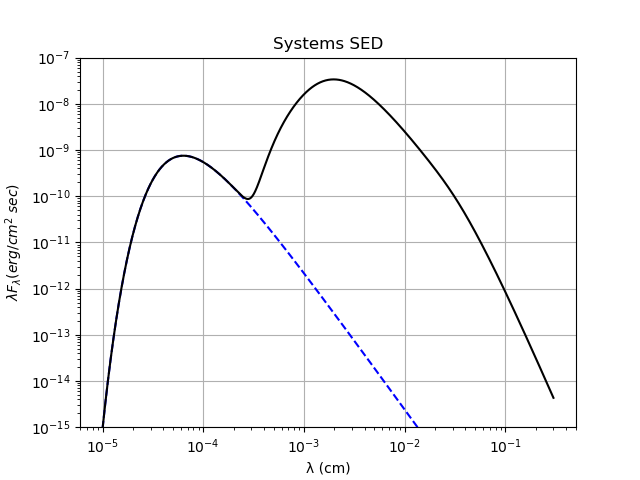
\includegraphics[scale=0.55]{SystemsSED.png}
\caption{Φασματική Κατανομή Ακτινοβολίας του Συστήματος Ήλιου-Δίσκου}\label{fig:SystemSED1}
\end{figure}

Παρακάτω σημειώνεται το όριο απο το οποίο και μετά ανιχνεύεται η παρουσία του δίσκου.


\begin{figure}[h]
\centering
 \begin{subfigure}{0.48\textwidth}
  \centering
  \includegraphics[width=\linewidth]{SystemsSED2.png}
  \caption{{\en System's SED 2}}\label{fig:SystemSED2}
 \end{subfigure}\hfill
 \begin{subfigure}{0.48\textwidth}
  \centering
  \includegraphics[width=\linewidth]{SystemsSED3.png}
  \caption{{\en System's SED 3}}\label{fig:SystemSED3}
 \end{subfigure}
  \caption{Φασματική Κατανομή Ακτινοβολίας του Συστήματος Ήλιου-Δίσκου-2}
\end{figure}


Παρατηρώντας την \ref{fig:SystemSED1} διακρίνουμε δύο κορυφές. Η πρώτη αντιστοιχεί στον αστέρα, ενώ η ύπαρξη της δεύτερης μας φανερώνει ότι πέρα απο το αστέρι του συστήματος υπάρχει και ένας δίσκος μεσοαστρικής ύλης. Η συνάρτηση πηγής του δίσκου είναι μέλαν σώμα, αλλά η αναδυόμενη ειδική ένταση της ακτινοβολίας του, σε αντίθεση με του αστεριού, είναι πολλαπλασιασμένη με τον όρο του οπτικού βάθους \ref{eq:MonochromaticFlux}. Ακόμα η δεύτερη κορυφή είναι μετατοπισμένη σε μεγαλύτερα μήκη κύματος λόγω της πολύ μικρότερης θερμοκρασίας της μεσοαστρικής ύλης του δίσκου.\\

Στην γραφική παράσταση της {\en SED} υπολογίζουμε το γινόμενο $\lambda F_{\lambda}$ και όπως αναφέραμε, ο δισκος εκπέμπει πιο αποτελεσματικά στα μεγάλα μήκη κύματος. Σαν αποτέλεσμα έχουμε μεγαλύτερη μετατόπιση προς τα θετικά του άξονα $y$ του τμήματος που αντιστοιχεί στον δίσκο έναντι αυτού που αντιστοιχεί στον αστέρα. Αυτό φανερώνεται και απο το διάγραμμα μονοχρωματικής ροής, $F_{\lambda} vs \lambda$ του συστήματος, όπου δεν πολλαπλασιάζεται η μονοχρωματική ροή με το μήκος κύματος:

\begin{figure}[h]
\centering
  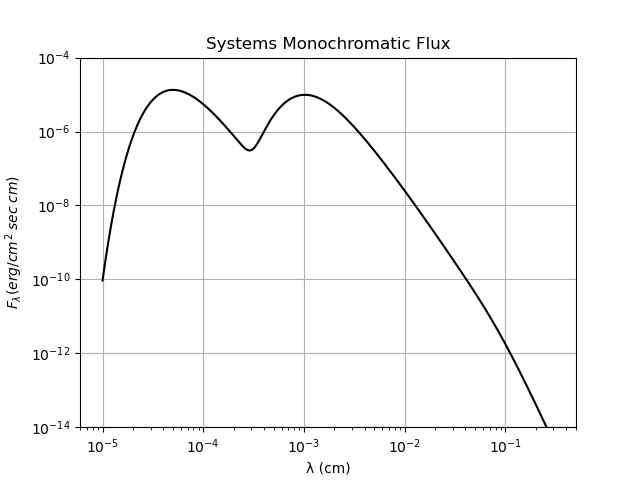
\includegraphics[scale=0.55]{SystemMonochromaticFlux.png}
\caption{Μονοχρωματική ροή ακτινοβολίας του συστήματος}\label{fig:SystemMonochromaticFlux}
\end{figure}


Στο σημείο αυτό πρέπει να αναλογιστούμε μια βασική υπόθεση που κάναμε για την απλοποίση του μοντέλου μας. Για τον υπολογισμό της {\it Θερμοκρασίας Ισορροπίας} της σκόνης θεωρήσαμε ότι {\bf ο δίσκος είναι οπτικά διαφανής} και κατ' επέκταση ότι η ακτινοβολία που απορροφάνε και επανεκπέμπουν τα σωματίδια της σκόνης δεν αποκόπτεται απο άλλα σωματίδια που πιθανώς βρίσκονται μπροστά απο τα πρώτα. Η παραπάνω υπόθεση καταλήγει στις μέγιστες θερμοκρασίες που μπορεί να έχει η σκόνη υπό την ακτινοβολία του συγκεκριμένου αστεριού άρα και στη μέγιστη μονοχρωματική ροή ακτινοβολίας που μπορεί να εκπέμψει αυτός ο δίσκος. Μια πιο αυστηρή ανάλυση του προβλήματος απαιτεί την λύση της διάδοσης της ακτινοβολίας μέσα στον δίσκο. \\

Παρακάτω δίνονται οι γραφικές παραστάσεις της μονοχρωματικής ροής του αστέρα και του δίσκου, για 1000 σημεία με $\lambda$ απο $0.1$μ$m$ έως $3000mm$ (σε λογαριθμική κλιμακα), δίνονται παρακάτω:

\begin{figure}[h]
\centering
 \begin{subfigure}{0.48\textwidth}
  \centering
  \includegraphics[width=\linewidth]{SunMonochromaticFlux.png}
  \caption{Φασματική Κατανομή Ακτινοβολίας του Ήλιου}\label{fig:SunMonochromaticFlux}
 \end{subfigure}\hfill
 \begin{subfigure}{0.48\textwidth}
  \centering
  \includegraphics[width=\linewidth]{DiscMonochromaticFlux.png}
  \caption{Φασματική Κατανομή Ακτινοβολίας του Δίσκου}\label{fig:DiscMonochromaticFlux}
 \end{subfigure}
\end{figure}

και δίνονται αντίστοιχα σε $mJy$, μέσω του {\en script: {\it FluxmJy.py}}:

\begin{figure}[h]
\centering
 \begin{subfigure}{0.48\textwidth}
  \centering
  \includegraphics[width=\linewidth]{SunMonchromaticFluxJY.png}
  \caption{Φασματική Κατανομή Ακτινοβολίας του Ήλιου σε {\en mJy}}\label{fig:SunFluxJy}
 \end{subfigure}\hfill
 \begin{subfigure}{0.48\textwidth}
  \centering
  \includegraphics[width=\linewidth]{DiscMonchromaticFluxJY.png}
  \caption{Φασματική Κατανομή Ακτινοβολίας του Δίσκου σε {\en mJy}}\label{fig:DiscFluxJy}
 \end{subfigure}
\end{figure}

Το εμβαδόν της καμπύλης των διαγραμμάτων μας δίνει την συνολική ροή του αστέρα και του δίσκου αντίστοιχα στην απόσταση των $100pc$ (\ref{eq:FluxBolMon}).
Η συνολική ροή για τον Ήλιο προκύπτει $1.027\times10^{-9} \frac{erg}{sec \; cm^2}$, ενώ για τον δίσκο $5.173\times10^{-8} \frac{erg}{sec \; cm^2}$. Βλέπουμε δηλαδή ότι η ροή του δίσκου φαίνεται να είναι $\sim50$ φορές μεγαλύτερη απο του αστέρα.\\

Αν θυμηθούμε το προφίλ της επιφανειακής πυκνότητας του δίσκου, \ref{fig:SurfDens}, βλέπουμε ότι η μάζα στον δίσκο κατανέμεται με τέτοιον τρόπο ώστε το 55.25\% της συνολικής μάζας του δίσκου βρίσκεται μεταξύ $1-5 AU$, δηλαδή σε έναν δακτύλιο εύρους $~4AU$. Προφανώς και όταν μια τόσο μεγάλη μάζα σκόνης ($5.525\times10^{-4} Μ_{\odot}$) κατανέμεται σε μια τόσο μικρή περιοχή η προσέγγιση του μικρού οπτικού βάθους ξεκινάει να κλονίζεται. Ακόμα παρατηρώντας το προφίλ κατανομής των θερμοκρασιών του δίσκου, \ref{fig:DiscTemp}, βλέπουμε ότι η παραπάνω περιοχή του δίσκου αντιστοιχεί και στην περιοχή με τις μεγαλύτερες θερμοκρασίες. Έτσι ενώ μια {\it ομοιόμορφη} αύξηση της μάζας του δίσκου αυξάνει αναλογικά την ροή, η ταυτόχρονη αύξηση του οπτικού βάθους θα έπρεπε να μειώνει την θερμοκρασία ισορροπίας της σκόνης. Απο την εξίσωση \eqref{eq:TotalPossitiveFlux} βλεπουμε ότι η ροή εξαρτάται εκθετικά απο την θερμοκρασία, οπότε ακόμα και μια μικρή διόρθωση στην τιμή της θερμοκρασίας επηρεάζει σημαντικά την ροη.\\

Στο σημείο αυτό χωρίσαμε τον δίσκο σε δύο περιοχές απο $1-5AU$ και απο $5-20.4AU$ και μετρήσαμε την μονοχρωματική ροή του κάθε τμήματος προσεγγίζοντας τα σαν δύο διαφορετικά σώματα απο το εμβαδόν της κάθε καμπύλης. Παρακάτω δίνονται οι γραφικές παραστάσεις της μονοχρωματικής ροής των δύο περιοχών αντίστοιχα:

\begin{figure}[h]
\centering
 \begin{subfigure}{0.48\textwidth}
  \centering
  \includegraphics[width=\linewidth]{Disc0-5AUMonochromaticFlux.png}
  \caption{Μονοχρωματική ροή ακτινοβολίας απο το κομμάτι του δίσκου 0-5{\en AU}}\label{fig:DiscMonochromaticFlux1stPart}
 \end{subfigure}\hfill
 \begin{subfigure}{0.48\textwidth}
  \centering
  \includegraphics[width=\linewidth]{Disc5-20AUMonochromaticFlux.png}
  \caption{Μονοχρωματική ροή ακτινοβολίας απο το κομμάτι του δίσκου 5-20.4{\en AU}}\label{fig:DiscMonochromaticFlux2ndPart}
 \end{subfigure}
\end{figure}

Οι συνολικές ροές που μετρήθηκαν είναι $1.6\times10^{-8} \frac{erg}{sec \; cm^2}$ και $3.57\times10^{-8} \frac{erg}{sec \; cm^2}$ για το πρώτο και το δεύτερο τμήμα αντίστοιχα. Βλέπουμε ότι η ροή απο το δεύτερο τμήμα είναι $\sim2.23$ φορές μεγαλύτερη απο αυτή του πρώτου! Αρκεί να αναλογιστούμε το εξης:\\

Εάν ο δίσκος ήταν \underline{απόλυτα οπτικά διαφανής} θα έπρεπε το πρώτο κομμάτι του έχοντας μεγαλύτερη μέση θερμοκρασία και ταυτόχρονα μεγαλύτερη επιφανειακή πυκνότητα να έχει μεγαλύτερη ροή. Ο λόγος που αυτό δεν παρατηρείται προδίδεται απο τις εξίσωσεις \ref{eq:MonochromaticFlux} και \ref{eq:OpticalDepth3}, όπου οι μεγάλες τιμές επιφανειακής πυκνότητας σε συνδυασμό με την μικρότερη ροή σε σχέση με το δεύτερο κομμάτι του δίσκου μας λέει ότι τελικά {\it δεν και τόσο οπτικά διαφανής} και μάλιστα το πρώτο κομμάτι είναι περισσότερο αδιαφανή απο το δεύτερο. Ουσιαστικά επιβεβαιώνεται ότι η προσέγγιση του μικρού οπτικού βάθους εισάγει ένα σφάλμα στην μέτρηση της θερμοκρασίας ισορροπίας της σκόνης, το οποίο είναι μεγαλύτερο για το πρώτο κομμάτι του δίσκου και μικρότερο για το δεύτερο.\\

Όσον αφορά την ροή που λαμβάνουμε απο τον Ήλιο, μπορούμε να επαληθεύσουμε την τιμή της. Το μέγιστο της γραφικής παράστασης \ref{fig:SunMonochromaticFlux} αντιστοιχεί στο $\lambda = 0.000050002 cm = 0.5002$μ$m$ και απο τον νόμο του {\en Wien}, \eqref{eq:WienLaw},  προκύπτει η θερμοκρασία του 'Ηλιο $T_{Sun}= 5793.68 K$. Η τιμή είναι πολύ κοντά στην τιμή, \ref{eq:SunsTemp}, που μετρήσαμε και η απόκλιση της προκύπτει απο το γεγονός ότι εδώ εξετάσαμε την μονοχρωματική ροή σε συγκεκριμένο εύρος μηκών κύματος και όχι την βολομετρική που αντιστοιχεί σε όλο το φάσμα. Ακόμα απο το εμβαδόν του ολοκληρώματος υπολογίσαμε ότι η μονοχρωματική ροή του Ήλιου στα $100pc$ είναι $1.027\times10^{-9} \frac{erg}{sec \; cm^2}$. Απο την \ref{eq:Brightness2} και \ref{eq:TotalInteBlackBody} για $100pc$ προκύπτει:

\begin{align*}
\frac{L_\odot}{4\pi (100 pc)^2} = \pi F_\lambda \Rightarrow\\
F_\lambda = \frac{3.8412 \times 10^{33}}{4\pi^2\times(100\times206265\times1.4959^{13})^2} \Rightarrow\\
F_\lambda = 1.022\times10^{-9} \frac{erg}{sec \; cm^2}
\end{align*}

όπου η τιμή μας επαληθεύεται με πάρα πολυ καλή ακρίβεια. \\

Συνοψίζοντας, βλέποντας και μόνο την {\en SED} \ref{fig:SystemSED1} μπορούμε να πούμε τα εξής:

\begin{itemize}

\item Η μορφή της {\en SED} προδίδει την ύπαρξη πρωτοπλανητικού δίσκου γύρω απο τον αστέρα.
\item O πρωτοπλανητικός δίσκος έχει μικρότερη μέση θερμοκρασία απο τον αστέρα.
\item O πρωτοπλανητικός δίσκος εκπέμπει το μεγαλύτερο μέρος της ενέργειας του στα μεγαλύτερα μήκη κύματος.
\item Η υπόθεση οπτικής διαφάνειας οδηγεί στις μέγιστες θερμοκρασίες για τον δίσκο και κατ' επέκταση στην μέγιστη εκπεμπόμενη μονοχρωματική ροή.
\end{itemize}
\newpage


\section{Κατανομή Λαμπρότητας}

Παρατηρώντας την {\en SED} του συστήματος, \ref{fig:SystemSED1}, εντοπίζουμε την ύπαρξη του δίσκου με τα χαρακτηριστικά που αναφέρθηκαν, αλλα η παρουσία του πλανήτη δεν είναι ακόμα προφανής. Όπως αναφέρθηκε στο κεφάλαιο 3, η <<υπογραφή>> της ύπαρξης του πλανήτη είναι η ύπαρξη συντονισμών μέσης κίνησης αλλά και ο κενός δακτύλιος που δημιουργεί στην τροχιά του σε συνδυασμό με την μη ισοτροπική κατανομή των {\en test paticles} κοντά στην απόσταση $r$ του πλανήτη. Κατ' επέκταση οι δύο ομάδες των {\en test particles} που ακολουθούν την τροχιά του (που βρίσκονται σε συντονισμό $1:1$ με αυτόν) και εντοπίζονται στα {σημεία ευσταθούς ισορροπίας {\en Lagrange}} $L_4$ και $L_5$. Στο σημείο αυτό θα προσπαθήσουμε να δημιουργήσουμε δισδιάστατες απεικονίσεις του συστήματος μέσω  της μονοχρωματικής ακτινοβολίας που λαμβάνουμε σε διάφορες συχνότητες παρατήρησης, ώστε να αναδείξουμε αυτην την γεωμετρία του σύστηματος και να έχουμε άμεση απόδειξη της ύπαρξης του πλανήτη.\\

Για την δημιουργία των απεικονίσεων ή <<φωτογραφιών>> συντάχθηκε ένα {\en script} με την ονομασία {\en {\it 2DImageArcsecAU.py}}, όπου χωρίσαμε τον δίσκο σε {\en ``pixels``}, αριθμού $i \times j$ και διαστάσεων $\Delta x^i$, $\Delta y^j$. Φυσικά όσο μεγαλύτερος είναι ο αριθμός των {\en ``pixels``} τόσο μικρότερο είναι και το μέγεθος τους. Ο αριθμός τους δεν μπορεί να είναι απεριόριστα μεγάλος καθώς αυτό θα συνεπάγεται ελάχιστο έως μηδενικό αριθμό σωματιδίων εντός του κάθε {\en ``pixel``} εισάγοντας με αυτόν τον τρόπο ένα στατιστικό σφάλμα. Στη συνέχεια μετρήσαμε όχι μόνο την μέση θερμοκρασία του κάθε {\en ``pixel``} η οποία εξαρτάται μόνο απο την απόσταση του απο το κέντρο του δίσκου \eqref{eq:DustTemp}, αλλά και όλα τα {\en test particles} εντός αυτών. Έπειτα γνωρίζοντας την επιφάνεια του κάθε {\en ``pixel``}, τον αριθμό των {\en test particles} εντός αυτού αλλα και την μάζα του κάθε {\en test particle} \eqref{eq:InitialTPMass} υπολογίσαμε την επιφανειακή πυκνότητα μάζας του κάθε {\en ``pixel``}. Έτσι η μονοχρωματική ροή του κάθε {\en ``pixel``} ($mJy$), σε συνδυασμό με την \eqref{eq:MonochromaticFlux}, δίνεται ώς:

\begin{equation}\label{eq:PixelFlux}
  F_{\nu}^{[i,j]} = (\frac{\Delta x^i \Delta y^j}{D^2})(1-e^{-\tau_{\nu}^{[i,j]}})B_{\nu}(Τ_{dust}^{[i,j]})
\end{equation}
και
\begin{equation}\label{eq:OpticalDepth4}
  \tau_{\nu,[i,j]} = 0.3821 (\frac{\nu}{\nu_0})^{2} \Sigma_{[i,j]},\; \text{όπου $\Sigma_{[i,j]}$ σε $\frac{g}{cm^{2}}$}
\end{equation}

Είναι σύνηθες να βλέπουμε την μονοχρωματική ροή σε μονάδες  $mJy/beam$, όπου $beam$ είναι η συνθετική ακτίνα του ραδιοτηλεσκοπίου εντός της οποίας γίνεται η μέτρηση. Στην συγκεκριμένη εργασία χρησιμοποιήσαμε μια $Gaussian \; beam$, το μέγεθος της οποίας καθορίζεται απο το {\en FWHM} και δίνεται σε $arcsec$. Το μέγεθος της ακτίνας δίνεται απο την \eqref{eq:GaussianBeam} και για τον λόγο αυτό το {\en {\it 2DImageArcsecAU.py}} συντάχθηκε με τέτοιο τρόπο ώστε να μας δίνει τη δυνατότητα να μετράμε το μέγεθος των {\en ``pixels``} είτε σε $AU$ είτε σε $arcsec$. Για να πάμε απο $mJy$ σε $mJy/beam$ ξεκινάμε απο την \eqref{eq:PixelFlux}:

\begin{align}
 F_{\nu}^{[i,j]} = (\frac{\Delta x^i \Delta y^j}{D^2})(1-e^{-\tau_{\nu}^{[i,j]}})B_{\nu}(Τ_{dust}^{[i,j]}) \; \text{$mJy$}\\
 F_{\nu}^{[i,j]} = \frac{\Delta\Omega_b(1-e^{-\tau_{\nu}^{[i,j]}})B_{\nu}(Τ_{dust}^{[i,j]})}{ 4.25\times10^{10}} \; \text{$mJy/beam$}
\end{align}\label{eq:PixelFluxBeam}
όπου $1 steradian = 4.25\times10^{10} (arcsec)^2$.

Τα διάφορα μεγέθη της συνθετικής δέσμης που χρησιμοποιήθηκαν για τις απεικονίσεις του δίσκου δίνονται στον πίνακα \ref{tab:ALMA}. Επιλέξαμε τις μικρότερες δυνατές τιμές του {\en FWHM} για τις διάφορες συχνότητες χωρίς όμως να αποκόπτουμε μέρος του δίσκου. Αυτο σημαίνει ότι φροντίσαμε ώστε η $\vartheta_{MRS}$ να είναι μεγαλύτερη απο την ακτινική διάμετρο του δίσκου ($\vartheta_{MRS}\geq0.408 arcsec$). Η επιλογή της στενής δέσμης γίνεται κατανοητή αν αναλογιστούμε το εξής: Απο την στιγμή που ο δίσκος χωρίστηκε σε {\en ``pixels``}, αριθμού $i \times j$ και διαστάσεων $\Delta x^i$, $\Delta y^j$, το μέγεθος του κάθε {\en pixel} σε $arcsec$ είναι γνωστό. Το εύρος του κενού δακτυλίου στον δίσκο αντιστοιχεί σε κάποιο αριθμό {\en ``pixels``} και κατ' επέκταση σε μια τιμή σε $arcsec$. Ακόμα το εύρος της δέσμης, σε $arcsec$, για τις διάφορες συχνότητες είναι επίσης γνωστό απο την \eqref{eq:GaussianBeam} και τον πίνακα \ref{tab:ALMA}. Έτσι, αφού η τελική εικόνα που προκύπτει είναι η {\it συνέλιξη της δέσμης του ραδιοσυμβολόμετρου με την διασδιάστατο πίνακα μονοχρωματικής ροής}, αν το μέγεθος της δέσμης είναι μικρότερο ή οριακά ίσο με το εύρος του κενού δακτυλίου, τότε αυτός θα είναι απόλυτα ορατός. Στην περίπτωση που η δεσμη είναι μεγαλύτερη απο τον κενό δακτύλιο η διαδικασία της συνέλιξης θα δώσει μια εικόνα στην οποία ο κενός δακτύλιος θα είναι λιγότερο ορατός ή μπορεί να μην είναι και καθόλου ορατός, διότι θα υπάρχει κάποια τιμή μονοχρωματικής ροής στα συγκεκριμένα {\en ``pixels``} λόγω του {\en averaging} που γίνεται εντός της δέσμης. Ακόμα θα πρέπει να προσέξουμε ώστε το μέγεθος της δέσμης να αντιστοιχεί τουλαχιστον σε 16 {\en ``pixels``}, ώστε να μην χάνεται πληροφορία λόγω φτωχής <<ψηφιοποίησης>> της δέσμης συνέλιξης. Η εκλογή περισσότερων {\en ``pixels``} συνεπάγεται την καλύτερη αναπαράσταση της συνθετικής δέσμης του ραδιοτηλεσκοπίου με την οποία συνελίσουμε την πρωτογεννή εικόνα. Παρακάτω δίνονται εικόνες του δίσκου, στις διάφορες τιμές συχνότητας , αλλά και για τα αντίστοιχα μεγέθη της δέσμης που αναγράφονται στον πίνακα \ref{tab:ALMA} πριν και μετα την συνέλιξη με την δέσμη:

\begin{figure}[h]
\centering
 \begin{subfigure}{0.33\textwidth}
  \centering
  \includegraphics[width=\linewidth]{870Unconv.png}
  \caption{{\en Unconvolved Disc at 100pc}}\label{fig:870gHzUnconvolved}
 \end{subfigure}\hfill
 \begin{subfigure}{0.33\textwidth}
  \centering
  \includegraphics[width=\linewidth]{870Conv.png}
  \caption{{\en Disc at 100pc}}\label{fig:870gHzCOnvolved}
 \end{subfigure}\hfill
 \begin{subfigure}{0.33\textwidth}
  \centering
  \includegraphics[width=\linewidth]{870ConvLog.png}
  \caption{{\en Disc at 100pc-Log Flux Density}}\label{fig:Log870gHzCOnvolved}
 \end{subfigure}\hfill
  \caption{Απεικόνιση του δίσκου απόστασης $100pc$ στα $870GHz$}
\medskip
\centering
 \begin{subfigure}{0.33\textwidth}
  \centering
  \includegraphics[width=\linewidth]{650Unconv.png}
  \caption{{\en Unconvolved Disc at 100pc}}\label{fig:650gHzUnconvolved}
 \end{subfigure}\hfill
 \begin{subfigure}{0.33\textwidth}
  \centering
  \includegraphics[width=\linewidth]{650Conv.png}
  \caption{{\en Disc at 100pc}}\label{fig:650gHzCOnvolved}
 \end{subfigure}\hfill
 \begin{subfigure}{0.33\textwidth}
  \centering
  \includegraphics[width=\linewidth]{650ConvLog.png}
  \caption{{\en Disc at 100pc-Log Flux Density}}\label{fig:Log650gHzCOnvolved}
 \end{subfigure}\hfill
  \caption{Απεικόνιση του δίσκου απόστασης $100pc$ στα $650GHz$}
\end{figure}

\newpage

\begin{figure}[h]
\centering
 \begin{subfigure}{0.33\textwidth}
  \centering
  \includegraphics[width=\linewidth]{460Unconv.png}
  \caption{{\en Unconvolved Disc at 100pc}}\label{fig:460gHzUnconvolved}
 \end{subfigure}\hfill
 \begin{subfigure}{0.33\textwidth}
  \centering
  \includegraphics[width=\linewidth]{460Conv.png}
  \caption{{\en Disc at 100pc}}\label{fig:460gHzCOnvolved}
 \end{subfigure}\hfill
 \begin{subfigure}{0.33\textwidth}
  \centering
  \includegraphics[width=\linewidth]{460ConvLog.png}
  \caption{{\en Disc at 100pc-Log Flux Density}}\label{fig:Log460gHzCOnvolved}
 \end{subfigure}\hfill
  \caption{Απεικόνιση του δίσκου απόστασης $100pc$ στα $460GHz$}
\medskip
\centering
 \begin{subfigure}{0.33\textwidth}
  \centering
  \includegraphics[width=\linewidth]{325Unconv.png}
  \caption{{\en Unconvolved Disc at 100pc}}\label{fig:325gHzUnconvolved}
 \end{subfigure}\hfill
 \begin{subfigure}{0.33\textwidth}
  \centering
  \includegraphics[width=\linewidth]{325Conv.png}
  \caption{{\en Disc at 100pc}}\label{fig:325gHzCOnvolved}
 \end{subfigure}\hfill
 \begin{subfigure}{0.33\textwidth}
  \centering
  \includegraphics[width=\linewidth]{325ConvLog.png}
  \caption{{\en Disc at 100pc-Log Flux Density}}\label{fig:Log325gHzCOnvolved}
 \end{subfigure}\hfill
  \caption{Απεικόνιση του δίσκου απόστασης $100pc$ στα $325GHz$}
  \medskip
\centering
 \begin{subfigure}{0.33\textwidth}
  \centering
  \includegraphics[width=\linewidth]{230Unconv.png}
  \caption{{\en Unconvolved Disc at 100pc}}\label{fig:230gHzUnconvolved}
 \end{subfigure}\hfill
 \begin{subfigure}{0.33\textwidth}
  \centering
  \includegraphics[width=\linewidth]{230Conv.png}
  \caption{{\en Disc at 100pc}}\label{fig:230gHzCOnvolved}
 \end{subfigure}\hfill
 \begin{subfigure}{0.33\textwidth}
  \centering
  \includegraphics[width=\linewidth]{230ConvLog.png}
  \caption{{\en Disc at 100pc-Log Flux Density}}\label{fig:Log230gHzCOnvolved}
 \end{subfigure}\hfill
  \caption{Απεικόνιση του δίσκου απόστασης $100pc$ στα $230GHz$}
\end{figure}

Βλέποντας τις παραπάνω εικόνες μπορούμε να κατανοήσουμε την σημασία της μεγάλης  διακριτικής ικανότητας για την ανάδειξη της γεωμετρίας του δίσκου με μεγαλύτερη λεπτομέρεια. Αν δούμε την περίπτωση της απεικόνισης στα $325GHz$, όπου έχουμε πολύ στενή δέσμη, ο κενός δακτύλιος είναι αρκετά εμφανής. Στην περίπτωση όμως της απεικονίσεως των $650GHz$ το εύρος της δέσμης είναι $\sim1.7$ φορές μεγαλύτερο$\cdot$ με αποτέλεσμα ο κενός δακτύλιος να είναι λιγότερο εμφανής.\\

Η ικανότητα μας να απεικονίσουμε τον κενό δακτύλιο με μεγαλύτερη λεπτομέρεια δεν σταματάει εδώ. Ας υποθέσουμε ότι έχουμε την παραπάνω εικόνα του δίσκου στα $325GHz$, η οποία απο μόνη της είναι ένα πολύ ισχυρό επιχείρημα για την ύπαρξη πλανήτη. Βλεπουμε ότι ο κενός δακτύλιος βρίσκεται εντός μιας γωνιακής διαμέτρου  $\sim 1 arcsec$ και απο τον πινακα \ref{tab:ALMA} βλεπουμε ότι $\vartheta_{MRS} = 0.418 arcsec$. Σαν αποτέλεσμα αν είχαμε πραγματικά την δυνατότητα χειρισμού του {\en ALMA} μετά την απεικόνιση του πλήρη δίσκου θα μπορούσαμε να επιλέξουμε ακόμα μικροτερες διακριτικές ικανότητες (με $\vartheta_{MRS} < 0.408 arcsec$) αποκόπτοντας μεν τα εξωτερικά όρια του δίσκου, αλλά λαμβάνοντας μεγαλύτερη λεπτομέρεια στην απεικόνιση του κενού το οποίο βρίσκεται εντός $\vartheta_{MRS}$. Ουσιαστικά στην περίπτωση αυτή το ραδιοσυμβολόμετρο αποκόπτει την μονοχρωματικη ροή που έρχεται απο $\vartheta_{MRS}$ και πάνω και σαν αντάλλαγμα παρέχει μεγαλύτερη διακριτική ικανότητα στην απεικόνιση της περιοχής $\vartheta_{MRS}$ και κάτω.\\

Μια ακόμα σημαντική βελτίωση στην λεπτομέρεια της εικόνας μπορεί να εισέλθει αυξάνοντας τον αριθμό των {\en ``pixels``} της εικόνας. Όπως αναφέραμε όσο μεγαλώνει ο αριθμός αυτός όλο και λιγότερα σωματίδια περιέχονται σε κάθε {\en ``pixel``} αυξάνοντας το στατιστικό σφάλμα στις μετρήσεις. Εύλογα μπορεί να συμπεράνει κανείς ότι περιοχές με μικρή επιφανειακή πυκνότητα θα παρουσιάζουν μεγαλύτερο στατιστικό σφάλμα έναντι αυτών με μεγαλύτερη. Στο σημείο αυτό εκμεταλλευόμαστε το ότι ο κενός δακτύλιος και κατ' επέκταση η περιοχή που θέλουμε να απεικονίσουμε είναι η εσωτερική περιοχή του δίσκου και εντοπίζεται σε γωνιακή διαμέτρο $\leq 1 arcsec$. Σαν αποτέλεσμα αυξάνοντας των αριθμό των {\en ``pixels``} της εικόνας αυξάνεται περισσότερο το στατιστικό σφάλμα των περιοχών γωνιακής διαμέτρου $> 1 arcsec$, αλλα οι περιοχές αυτές γίνονται {\en ``filter-out``} λόγω του ορίου που θέτει η $\vartheta_{MRS}$. Παρακάτω δίνονται οι εικόνες του δίσκου στα $325GHz$ και $230GHz$ και τα αντίστοιχα μεγέθη της δέσμης που αναγράφονται στον πίνακα \ref{tab:ALMA2}. Παρέχονται εικόνες μετα την συνέλιξη με την δέσμη:

\begin{figure}[h]
\centering
 \begin{subfigure}{0.48\textwidth}
  \centering
  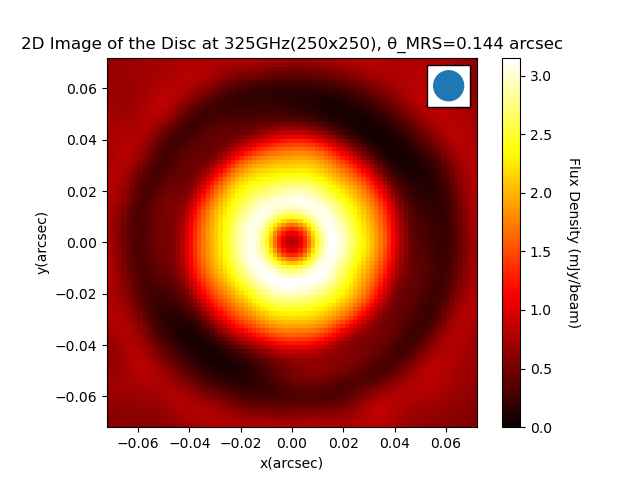
\includegraphics[width=\linewidth]{325ConvThMRS.png}
  \caption{{\en Disc at 100pc}, $\vartheta_{MRS}= 0.144 arcsec$}\label{fig:325ConvThMRS}
 \end{subfigure}\hfill
 \begin{subfigure}{0.48\textwidth}
  \centering
  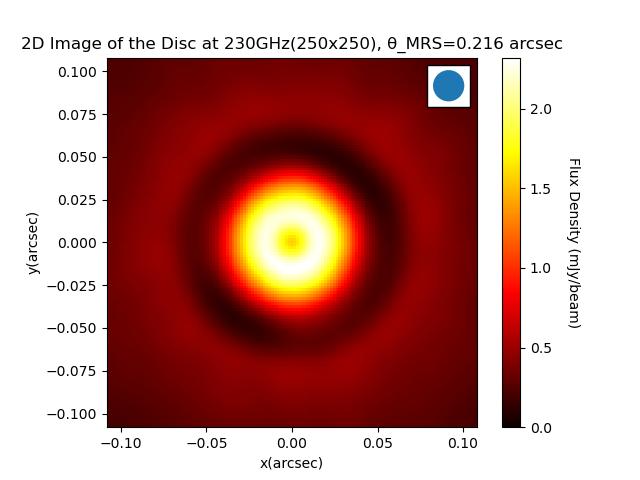
\includegraphics[width=\linewidth]{230ConvThMRS.png}
  \caption{{\en Disc at 100pc}, $\vartheta_{MRS}= 0.216 arcsec$}\label{fig:230ConvThMRS}
 \end{subfigure}\hfill
 \caption{Απεικόνιση εσωτερικού τμήματος του δίσκου απόστασης $100pc$}
\end{figure} 

Στις παραπάνω εικόνες βλέπουμε με πολύ μεγάλη ευκρίνεια τον κενό δακτύλιο, ο οποίος αποτελεί και την \underline{ένδειξη υπαρξης του πλανήτη.} Μάλιστα στην απεικόνιση των $325GHz$, όπου έχουμε και την μεγαλύτερη δυνατή διακριτική ικανότητα, μπορούμε να διακρίνουμε αμυδρά τις δύο ομάδες των αντίστοιχων Τρωικών. Φυσικά θα πρέπει κανείς να σκεφτεί ότι σε μια πραγματική απεικόνιση ενός δίσκου θα υπάρχει και θερμικός θόρυβος, ο οποίος <<θολωνει>> την εικόνα. Σαν αποτέλεσμα οι πραγματικές απεικονίσεις θα είναι πιο θολές και με μικρότερη λεπτομέρεια. Πιθανότατα να μην φαίνονται οι Τρωικοί δορυφόροι, αλλα {\it η ύπαρξη και μόνο του κενού δακτυλίου είναι η <<υπογραφή>> της παρουσίας του γιγάντιου πλανήτη στο σύστημα.}\\

Τέλος μπορεί να παρατηρήσει κανείς ότι τελίκά επιλέξαμε τις μικρότερες συχνότητες για την απεικόνιση του δίσκου και η επιλογή αυτή δεν είναι τυχαία. Αρχικά βλεπουμε ότι το {\en ALMA} μπορεί να πετύχει μεγαλύτερες διακριτικές ικανότητες σε αυτές τις συχνότητες μέσω των {\en Configurations C-10}. Ο δεύτερος και πιο σημαντικός λόγος είναι ότι όπως αποδείξαμε η σκόνη εκπέμπει πιο αποτελεσματικά στα μεγαλύτερα μήκη κύματος έναντι του αστέρα. Μικρότερες συχνότητες ισοδυναμούν με μεγαλύτερα μήκη κύματος, άρα σε μια πραγματική απεικόνιση, όπου θα περιεχόταν και το αστέρι στο κέντρο του δίσκου, η μονοχρωματική ακτινοβολία που θα λαμβάναμε απο αυτό θα είναι σημαντικά μικρότερη έναντι του δίσκου. Σαν αποτέλεσμα είναι δυνατό να εντοπίσουμε τις δομικές λεπτομέρειες του δίσκου χώρις η φασματική κατανομή ακτινοβολίας του αστέρα να κυριαρχεί. Εάν το τελευταίο συνέβαινε τότε θα ήταν αναγκαίες μη πραγματοποιήσιμες απεικονίσεις με μεγάλο δυναμικό εύρος, ώστε να μπορούσε να αποκαλυφθεί ο δίσκος και τα δυναμικά χαρακτηριστικά του, τα οποία μας δείχνουν την ύπαρξη του μαζικού πλανήτη.